\documentclass[11pt, spanish, a4paper, twoside]{article}
% LTeX: language=es-AR

% Versión 1.er cuat 2021 Víctor Bettachini < vbettachini@unlam.edu.ar >

\usepackage[T1]{fontenc}
\usepackage[utf8]{inputenc}

\usepackage[spanish, es-tabla]{babel}
% \def\spanishoptions{argentina} % Was macht dass?
% \usepackage{babelbib}
% \selectbiblanguage{spanish}
% \addto\shorthandsspanish{\spanishdeactivate{~<>}}


\usepackage{graphicx}
\graphicspath{{./figuras/}{../LaTeX/}{../figurasLaTeX/}{./figs}}
% \usepackage{float}

\usepackage[arrowdel]{physics}
\newcommand{\pvec}[1]{\vec{#1}\mkern2mu\vphantom{#1}}
% \usepackage{units}
\usepackage[separate-uncertainty= true, multi-part-units= single, range-units= single, range-phrase= {~a~}, locale= FR]{siunitx}
\usepackage{isotope} % $\isotope[A][Z]{X}\to\isotope[A-4][Z-2]{Y}+\isotope[4][2]{\alpha}

\usepackage{tasks}
\usepackage[inline]{enumitem}
% \usepackage{enumerate}

\usepackage{hyperref}

% \usepackage{amsmath}
% \usepackage{amstext}
% \usepackage{amssymb}

\usepackage{tikz}
\usepackage{tikz-3dplot}
\usepackage{tikz-dimline}
\usetikzlibrary{calc}
% \usetikzlibrary{math}
\usetikzlibrary{arrows.meta}
\usetikzlibrary{snakes}
\usetikzlibrary{decorations}
\usetikzlibrary{decorations.pathmorphing}
\usetikzlibrary{patterns}

\usepackage[hmargin=1cm,vmargin=3cm, top= 0.75cm,nohead]{geometry}

\usepackage{lastpage}
\usepackage{fancyhdr}
\pagestyle{fancyplain}
\fancyhf{}
\setlength\headheight{28.7pt} 
\fancyhead[LE, LO]{\textbf{Mecánica Analítica Computacional} }
% \fancyhead[LE, LO]{\textbf{Mecánica General} }
\fancyhead[RE, RO]{\href{https://ingenieria.unlam.edu.ar/}{$\vcenter{\hbox{
\includegraphics[height=1cm]{ambos.pdf}}}$}}
\fancyfoot{\href{https://creativecommons.org/licenses/by-nc-sa/4.0/deed.es_ES}{$\vcenter{\hbox{
\includegraphics[height=0.4cm]{by-nc-sa_80x15.pdf}}}$} \href{https://ingenieria.unlam.edu.ar/}{DIIT - UNLaM}}
\fancyfoot[C]{ {\tiny Actualizado al \today} }
\fancyfoot[RO, LE]{Pág. \thepage/\pageref{LastPage}}
\renewcommand{\headrulewidth}{0pt}
\renewcommand{\footrulewidth}{0pt}

% LTeX: language = es-AR

\begin{document}
\begin{center}
  % \textsc{\large Mecánica general}\\
  \textsc{\large Cuerpo rígido | Tensores de inercia}
\end{center}

No se puede acceder a \textcolor{blue}{los URL de los enlaces en el texto marcado en azul}, desde el visor para PDF que provee GitHub.
Es necesario descargar este archivo hacíendo click en el ícono de descarga que se encuentra arriba a la derecha de la ventana que muestra el PDF. 
Luego en cualquier lector de PDF, incluso el del navegador, se puede hacer click en el texto en azul para que ser dirigido a la página del URL correspondiente.
% De poder resolver estos problemas en forma autónoma puede asumir que adquirió los conocimientos mínimos sobre los temas abordados en la semana. No dude en consultar a docentes y compañeros si no puede terminarlos.
% Los problemas marcados con (*) son opcionales.

\begin{enumerate}
	\item
	\textbf{Monóxido de carbono}\\
	Calcular el tensor de inercia de una molécula requiere conocer la distancia entre los átomos y sus masas.

	La distancia, o longitud de enlace, puede encontrarse en el \textcolor{blue}{\href{https://cccbdb.nist.gov/exp1x.asp}{buscador de propiedades de una molécula fruto de experimentos} de la \emph{Computational Chemistry Comparison and Benchmark DataBase} del National Institute of Standards and Technology, NIST, de los E.U.A}.
	Tras ingresar la fórmula química de la molécula, que en este caso es \emph{CO}, pueden encontrarse las distancias, o aún mejor las respectivas posiciones en un sistema de referencia cartesiano, expresadas en \si{angstrom}, equivalente a \SI{1e-10}{\metre}.

	La masa para cada elemento químico está expresada en unidades de masa atómica unificada, \si{\atomicmassunit} en la \textcolor{blue}{\href{https://iupac.org/what-we-do/periodic-table-of-elements/}{tabla periódica} publicada por la Unión Internacional de Química Pura y Aplicada, IUPAC}.
	Esta es la masa expresada en gramos de un mol de átomos con la proporción de isótopos que se presenta en la naturaleza.
	Para obtener la masa en gramos de uno sólo basta con dividirle por el número de átomos en este mol, la constante de Avogadro, \(N_A = \SI{6.022e23}{\per\mole}\).
	
	Expresar el tensor de inercia en unidades del SI (\si{\kilogram \squared \metre}).
	Resultado:\\
	\[
		\overline{\overline{I}} = \left[\begin{matrix}0 & 0 & 0\\0 & 1.45 \cdot 10^{-46} & 0\\0 & 0 & 1.45 \cdot 10^{-46}\end{matrix}\right]
	\]



	\item 
	\begin{minipage}[t][3cm]{0.73\textwidth}
	\textbf{Agua}\\
		Expresar el tensor de inercia en unidades del SI.
		Resultado:\\
		\[
			\overline{\overline{I}} = \left[\begin{matrix}1.02 \cdot 10^{-47} & 0 & 0\\0 & 1.92 \cdot 10^{-47} & 0\\0 & 0 & 2.95 \cdot 10^{-47}\end{matrix}\right]
		\]
	\end{minipage}
	\begin{minipage}[c][1cm][t]{0.2\textwidth}
		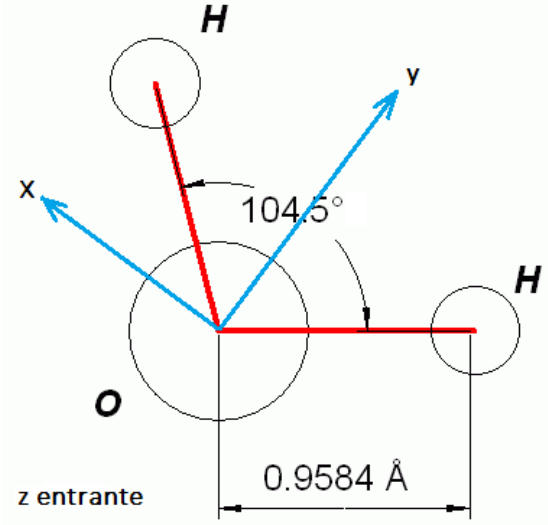
\includegraphics[width=\textwidth]{moleculaH2O}
	\end{minipage}

	

	\item 
	\begin{minipage}[t][3cm]{0.73\textwidth}
	\textbf{Diclorometano}\\
	Esta molécula tiene por fórmula química \isotope{CH_2Cl_2}. Expresar el tensor de inercia en unidades del SI.
		Resultado:\\
		\[
			\overline{\overline{I}} = \left[\begin{matrix}2.69 \cdot 10^{-46} & 0 & 0\\0 & 2.56 \cdot 10^{-45} & 0\\0 & 0 & 1.04 \cdot 10^{-36}\end{matrix}\right]
		\]
	\end{minipage}
	\begin{minipage}[c][0.5cm][t]{0.2\textwidth}
		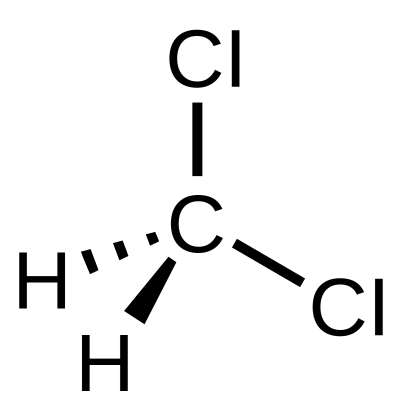
\includegraphics[width=\textwidth]{Dichloromethane_molecular_structure}
	\end{minipage}



	\item 
	\begin{minipage}[t][6cm]{0.65\textwidth}
		\textbf{Péndulo de torsión desbalanceado}\\
		El sistema que se muestra en la ilustración para \(t = 0 \) presenta pesos en los extremos de dos brazos.
		La barra dispuesta verticalmente se mantiene en tal dirección con rulemanes que posibilitan que el eje rote sin fricción con velocidad angular $\Omega$ constante respecto el marco inercial $O_{xyz}$.
		Para este análisis la masa de brazos y ejes es despreciable frente a la de los pesos \(m\).
		Calcule: 
		\begin{tasks} 
			\task tensor de inercia respecto a A en función del tiempo \(\overline{\overline{I}}_A(t)\)\\
			\task momento angular $\vec{L}_A (t) = \overline{\overline{I}}_A (t) \vec{\Omega}$ y torque $\vec{\tau} (t) = \dot{\vec{L}} (t)$.
		\end{tasks}
	\end{minipage}
	\begin{minipage}[c][0cm][t]{0.3\textwidth}
		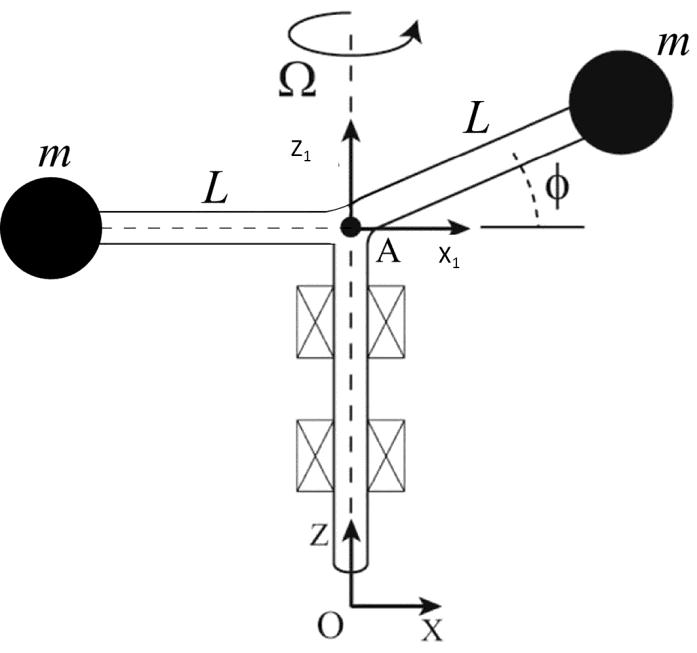
\includegraphics[width=\textwidth]{o-021}
	\end{minipage}
	Resultados:\\
			\[
				\scalebox{0.9}{$
				\overline{\overline{I}}_A = \left[\begin{matrix}\ell^{2} m \left(- \cos^{2}{\left(\phi \right)} \cos^{2}{\left(\Omega t \right)} - \cos^{2}{\left(\Omega t \right)} + 2\right) & - \ell^{2} m \left(\cos^{2}{\left(\phi \right)} + 1\right) \sin{\left(\Omega t \right)} \cos{\left(\Omega t \right)} & \frac{\ell^{2} m \left(\sin{\left(\Omega t - 2 \phi \right)} - \sin{\left(\Omega t + 2 \phi \right)}\right)}{4}\\- \ell^{2} m \left(\cos^{2}{\left(\phi \right)} + 1\right) \sin{\left(\Omega t \right)} \cos{\left(\Omega t \right)} & \ell^{2} m \left(\sin^{2}{\left(\phi \right)} \sin^{2}{\left(\Omega t \right)} - 2 \sin^{2}{\left(\Omega t \right)} + 2\right) & - \frac{\ell^{2} m \left(\cos{\left(\Omega t - 2 \phi \right)} - \cos{\left(\Omega t + 2 \phi \right)}\right)}{4}\\\frac{\ell^{2} m \left(\sin{\left(\Omega t - 2 \phi \right)} - \sin{\left(\Omega t + 2 \phi \right)}\right)}{4} & - \frac{\ell^{2} m \left(\cos{\left(\Omega t - 2 \phi \right)} - \cos{\left(\Omega t + 2 \phi \right)}\right)}{4} & \ell^{2} m \left(\cos^{2}{\left(\phi \right)} + 1\right)\end{matrix}\right]
				$}
				\] 
			\[
				\vec{L}_A = \left[\begin{matrix}\frac{\Omega \ell^{2} m \left(\sin{\left(\Omega t - 2 \phi \right)} - \sin{\left(\Omega t + 2 \phi \right)}\right)}{4}\\- \frac{\Omega \ell^{2} m \left(\cos{\left(\Omega t - 2 \phi \right)} - \cos{\left(\Omega t + 2 \phi \right)}\right)}{4}\\\Omega \ell^{2} m \left(\cos^{2}{\left(\phi \right)} + 1\right)\end{matrix}\right]
			\qquad
				\vec{\tau}_A = \left[\begin{matrix}\frac{\Omega^{2} \ell^{2} m \left(\cos{\left(\Omega t - 2 \phi \right)} - \cos{\left(\Omega t + 2 \phi \right)}\right)}{4}\\\frac{\Omega^{2} \ell^{2} m \left(\sin{\left(\Omega t - 2 \phi \right)} - \sin{\left(\Omega t + 2 \phi \right)}\right)}{4}\\0\end{matrix}\right]
			\]


	\end{enumerate}

\end{document}
